%%%%%%%%%%%%%%%%%%%%%%%%%%%%%%%%%%%%%%%%%
% Beamer Presentation
% LaTeX Template
% Version 1.0 (10/11/12)
%
% This template has been downloaded from:
% http://www.LaTeXTemplates.com
%
% License:
% CC BY-NC-SA 3.0 (http://creativecommons.org/licenses/by-nc-sa/3.0/)
%
%%%%%%%%%%%%%%%%%%%%%%%%%%%%%%%%%%%%%%%%%

%----------------------------------------------------------------------------------------
%	PACKAGES AND THEMES
%----------------------------------------------------------------------\------------------

\documentclass{beamer}
\usepackage{multicol}
\usepackage{xcolor}
\usepackage{listings}

\definecolor{applegreen}{rgb}{0.55, 0.71, 0.0}
\definecolor{blue(ncs)}{rgb}{0.0, 0.53, 0.74}
\definecolor{burgundy}{rgb}{0.5, 0.0, 0.13}

\mode<presentation> {

\usetheme{CambridgeUS}

\usecolortheme{wolverine}

\definecolor{gold}{HTML}{D4A017}
\definecolor{darkgold}{HTML}{B7950B}

\setbeamercolor{palette primary}{bg=gold,fg=white}
\setbeamercolor{palette secondary}{bg=darkgold,fg=white}
\setbeamercolor{palette tertiary}{bg=black,fg=white}
\setbeamercolor{palette quaternary}{bg=gold,fg=white}

\setbeamercolor{frametitle}{bg=darkgold,fg=white}

\setbeamercolor{section number projected}{bg=black,fg=gold}
\setbeamercolor{item}{fg=black,bg=gold}
}

\usepackage{graphicx} % Allows including images
\usepackage{booktabs} % Allows the use of \toprule, \midrule and \bottomrule in tables

%----------------------------------------------------------------------------------------
%	TITLE PAGE
%----------------------------------------------------------------------------------------

\title[Generic Finite Element Interfaces]{Designing Generic Finite Element Interfaces} % The short title appears at the bottom of every slide, the full title is only on the title page

\author{Jeremy L Thompson} % Your name
\institute[CU Boulder] % Your institution as it will appear on the bottom of every slide, may be shorthand to save space
{University of Colorado Boulder \\ % Your institution for the title page
\medskip
\textit{jeremy.thompson@colorado.edu} % Your email address
}
\date{\today} % Date, can be changed to a custom date

\begin{document}

\begin{frame}
\titlepage % Print the title page as the first slide
\end{frame}

%------------------------------------------------

\begin{frame}
\begin{center}
\frametitle{Overview}

A global sparse matrix is no longer a good representation of a\\high-order linear operator\\

~\\

libCEED is an extensible library that provides a portable\\algebraic interface and optimized implementations

\end{center}
\end{frame}
 
%------------------------------------------------

\begin{frame}
\frametitle{Overview} % Table of contents slide, comment this block out to remove it
\tableofcontents % Throughout your presentation, if you choose to use \section{} and \subsection{} commands, these will automatically be printed on this slide as an overview of your presentation
\end{frame}

%----------------------------------------------------------------------------------------
%	PRESENTATION SLIDES
%----------------------------------------------------------------------------------------

%------------------------------------------------
\section{Introduction}
%------------------------------------------------

%------------------------------------------------

\begin{frame}
\begin{center}
\frametitle{Fitite Elements Operator}

Finite elements discretizes the weak form of a PDE\\

~\\

Classical Form:\\
$- \Delta u = f$\\

~\\

Test Functions:\\
~\\

~\\

Weak Form:\\
~\\

~\\

Galerkin Form:\\
~

\end{center}
\end{frame}

%------------------------------------------------

\begin{frame}
\begin{center}
\frametitle{Fitite Elements Operator}

Finite elements discretizes the weak form of a PDE\\

~\\

Classical Form:\\
$- \Delta u = f$\\

~\\

Test Functions:\\
$- \int \varphi \Delta u = \int \varphi f$\\

~\\

Weak Form:\\
~\\

~\\

Galerkin Form:\\
~

\end{center}
\end{frame}

%------------------------------------------------

\begin{frame}
\begin{center}
\frametitle{Fitite Elements Operator}

Finite elements discretizes the weak form of a PDE\\

~\\

Classical Form:\\
$- \Delta u = f$\\

~\\

Test Functions:\\
$- \int \varphi \Delta u = \int \varphi f$\\

~\\

Weak Form:\\
$\int \nabla \varphi \nabla u = \int \varphi f$\\

~\\

Galerkin Form:\\
~

\end{center}
\end{frame}

%------------------------------------------------

\begin{frame}
\begin{center}
\frametitle{Fitite Elements Operator}

Finite elements discretizes the weak form of a PDE\\

~\\

Classical Form:\\
$- \Delta u = f$\\

~\\

Test Functions:\\
$- \int \varphi \Delta u = \int \varphi f$\\

~\\

Weak Form:\\
$\int \nabla \varphi \nabla u = \int \varphi f$\\

~\\

Galerkin Form:\\
$\int \nabla \varphi_i \nabla u = \int \varphi_i f$\\

$u = \sum_i c_i \varphi_i$

\end{center}
\end{frame}

%------------------------------------------------

\begin{frame}
\begin{center}
\frametitle{Operator Decomposition}

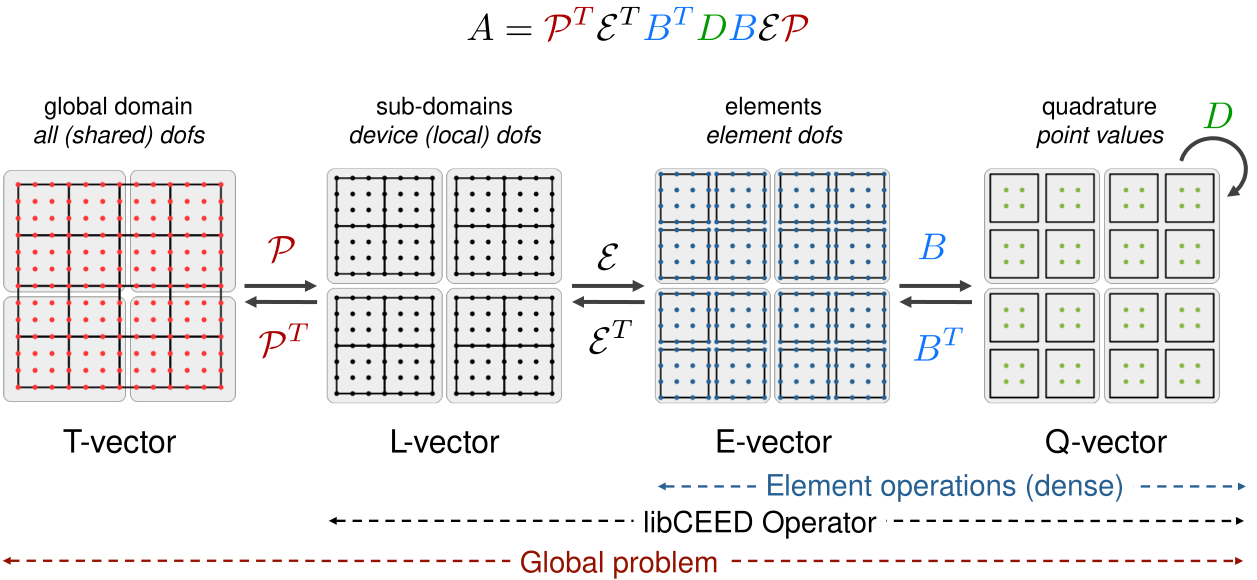
\includegraphics[width=11cm]{libCEEDAPI}

\end{center}
\end{frame}

%------------------------------------------------

\begin{frame}
\begin{center}
\frametitle{Assembled Matrix Cost!}

\begin{multicols}{2}

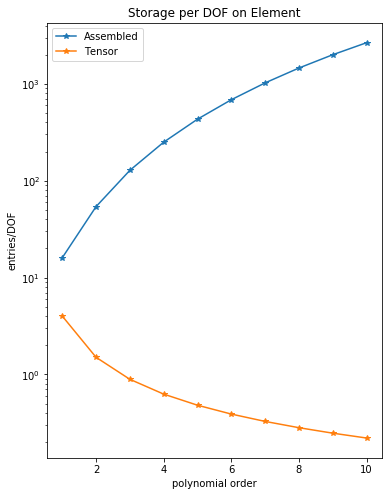
\includegraphics[height=5.5cm]{libCEEDAssembledVsTensorStoreage}\\

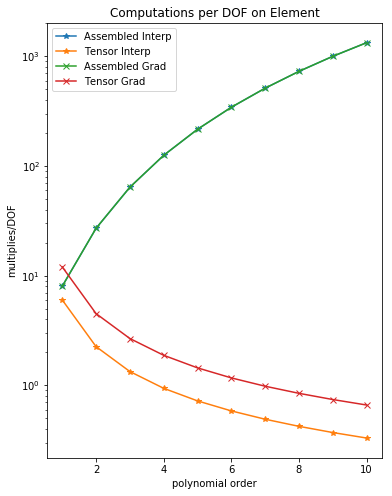
\includegraphics[height=5.5cm]{libCEEDAssembledVsTensorApply}

\end{multicols}

\end{center}
\end{frame}

%------------------------------------------------

\begin{frame}
\begin{center}
\frametitle{Matrix Free Implementation}

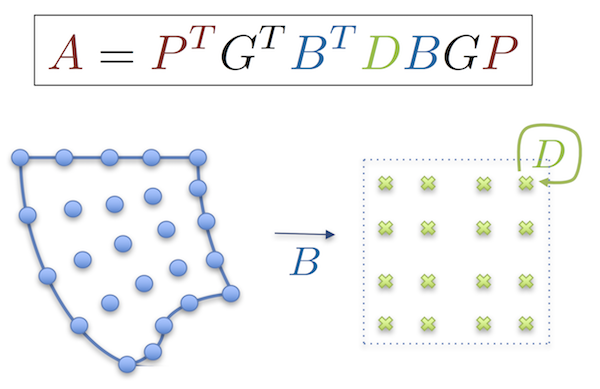
\includegraphics[width=5cm]{libCEEDRefElm}

\begin{itemize}

\item Avoid global matrix assembly

\item Map each element to reference element

\item Only store map to reference, action on reference

\item Easy to parallelize across nodes

\end{itemize}

\end{center}
\end{frame}

%------------------------------------------------
\section{libCEED}
%------------------------------------------------

\begin{frame}
\begin{center}
\frametitle{libCEED API}

\begin{itemize}

\item Provides on-device operator implementation\\

~\\

\item Easy to incorporate into existing code\\

~\\

\item Supports multiple types of computatinal devices\\

\begin{itemize}

\item CPU - Reference and vectorized, template for new backends

\item OCCA (jit) - CPU, OpenMP, OpenCL, and CUDA

\item MAGMA

\item One source code can call multiple CEEDs with different backends

\end{itemize}

\item v0.2 March and v0.3 (imminent)\\

\item BSD-2 license

\end{itemize}

\end{center}
\end{frame}

%------------------------------------------------

\begin{frame}
\begin{center}
\frametitle{API Objects}

\begin{itemize}

\item $G$ - CeedRestriction\\

\hspace{6mm} Restrict to single element\\

~\\

\item {\color{blue(ncs)} $B$} - CeedBasis\\

\hspace{6mm} Actions on basis such as interpolation,\\

\hspace{6mm} gradient, divergence, curl

~\\

\item {\color{applegreen} $D$} - CeedQFunction\\

\hspace{6mm} Operator action at quadrature points\\

\hspace{6mm} to include coefficient functions

\end{itemize}

\end{center}
\end{frame}

%------------------------------------------------

\begin{frame}
\begin{center}
\frametitle{Device Level Operator}

\begin{itemize}

\item $L = G^T {\color{blue(ncs)} B^T} {\color{applegreen} D} {\color{blue(ncs)} B} G$ - CeedOperator\\

~\\

\item libCEED objects are combined to create a CeedOperator\\

~\\

\item CeedOperator gives operator action for elements on device\\

~\\

\item User code responsible for communication between devices\\

\hspace{6mm} $A = {\color{burgundy} P^T} L {\color{burgundy} P}$

\end{itemize}

\end{center}
\end{frame}

%------------------------------------------------

\begin{frame}[fragile]
\begin{center}
\frametitle{Basis}

\begin{itemize}

\item Tensor $H^1$ elements\\

\item User provides $p, q, dim$ and chooses Gauss or Gauss-Lobatto dofs\\

\item Alternatively, user provides $1D$ interp, grad matrices and quadrature weights and points\\

\item More geometries, $H(div)$, $H(curl)$ coming\\

\end{itemize}

{\small
\begin{lstlisting}[language=C]

CeedBasisCreateTensorH1Lagrange(ceed, dim, ncomp,
                P, Q, CEED_GAUSS, &basis);
CeedBaisApply(basis, CEED_NOTRANSPOSE, CEED_EVAL_INTERP,
                x, xq);

\end{lstlisting}
}

\end{center}
\end{frame}

%------------------------------------------------

\begin{frame}[fragile]
\begin{center}
\frametitle{Restriction}

\begin{itemize}

\item Gather and scatter operations\\

\item Support conforming and non-conforming meshes\\

\item User provides index list, may be linear combination of dofs\\

\item On node communication only\\

\end{itemize}

{\small
\begin{lstlisting}[language=C]

CeedElemRestrictionCreate(ceed, ne, 2, ne+1, 1,
               CEED_MEM_HOST, CEED_USE_POINTER,
               ind, &rstr);
  CeedElemRestrictionApply(rstr, CEED_NOTRANSPOSE,
               CEED_NOTRANSPOSE, u, ru,
               CEED_REQUEST_IMMEDIATE);

\end{lstlisting}
}

\end{center}
\end{frame}

%------------------------------------------------

\begin{frame}[fragile]
\begin{center}
\frametitle{Qfunction}

\begin{itemize}

\item Applies the physics at the quadrature points\\

\item Multiple inputs and outputs\\

\end{itemize}

{\small
\begin{lstlisting}[language=C]

CeedQFunctionCreateInterior(ceed, 1, myfunc,
              __FILE__ ":myfunc", &qf);
CeedQFunctionAddInput(qf_setup, "_weight", 
              1, CEED_EVAL_WEIGHT);
CeedQFunctionAddInput(qf_setup, "x",
              1, CEED_EVAL_GRAD);
CeedQFunctionAddOutput(qf_setup, "rho",
              1, CEED_EVAL_NONE);

\end{lstlisting}
}

\end{center}
\end{frame}

%------------------------------------------------

\begin{frame}[fragile]
\begin{center}
\frametitle{Operator}

\begin{itemize}

\item Combines components to give local operator action\\

\item Multiple inputs and outputs\\

\item Composite operators coming\\

\end{itemize}

{\small
\begin{lstlisting}[language=C]

CeedOperatorCreate(ceed, qf_setup, NULL, NULL, &op_setup);

CeedOperatorSetField(op_setup, "_weight",
            CEED_RESTRICTION_IDENTITY, basis,
            CEED_VECTOR_NONE);
CeedOperatorSetField(op_setup, "x",
            rstr, basis, CEED_VECTOR_ACTIVE);
CeedOperatorSetField(op_setup, "rho",
            CEED_RESTRICTION_IDENTITY,
            CEED_BASIS_COLOCATED,
            CEED_VECTOR_ACTIVE);

\end{lstlisting}
}

\end{center}
\end{frame}

%------------------------------------------------

\begin{frame}
\begin{center}
\frametitle{Benefits}

\begin{itemize}

\item Extensible library\\

~\\

\item Lower memory transfer, no sparse matrix\\

~\\

\item Implementations for multiple devices and backends\\

~\\

\item Backend improvements benefit all applications\\

\hspace{6mm} Tensor contraction, basis application, etc

~\\

\item Minimal dependencies\\

\end{itemize}

\end{center}
\end{frame}

%------------------------------------------------
\section{Production Software}
%------------------------------------------------

\begin{frame}[fragile]
\begin{center}
\frametitle{Standalone Implementation}

\begin{lstlisting}[language=C]
  // Create the mass operator.
  CeedOperator oper;
  CeedOperatorCreate(CEED, apply_qfunc,
		NULL, NULL, &oper);

...

  // Apply the mass operator: 'u' -> 'v'.
  CeedOperatorApply(oper, u, v, 
		CEED_REQUEST_IMMEDIATE);
\end{lstlisting}

\end{center}
\end{frame}

%------------------------------------------------

\begin{frame}[fragile]
\begin{center}
\frametitle{MFEM}

{\small
\begin{lstlisting}[language=c++]
/// Wrapper for a mass CeedOperator as an
/// mfem::Operator
class CeedMassOperator : public mfem::Operator
 protected:
  const mfem::FiniteElementSpace *fes;
  CeedOperator build_oper, oper;
  CeedBasis basis, mesh_basis;
  CeedElemRestriction restr, mesh_restr;
  CeedQFunction apply_qfunc, build_qfunc;
  CeedVector node_coords, qdata;

\end{lstlisting}
}

\end{center}
\end{frame}

%------------------------------------------------

\begin{frame}[fragile]
\begin{center}
\frametitle{Nek5000}

{\small
\begin{lstlisting}[language=Fortran]
subroutine ceed_axhm1(pap,ap1,p1,h1,h2,ceed,op_mass,
$ vec_ap1,vec_p1,vec_qdata)

include 'ceedf.h'

c Vector conjugate gradient matvec for solution of 
c uncoupled Helmholtz equations

include 'SIZE'
include 'TOTAL'
...
call ceedvectorsetarray(vec_p1,ceed_mem_host,
$ ceed_use_pointer, p1,err)
call ceedoperatorapply(op_mass,vec_p1,vec_ap1,
$ ceed_request_immediate,err)
call ceedvectorgetarray(vec_ap1,ceed_mem_host,ap1,err)
\end{lstlisting}
}

\end{center}
\end{frame}

%------------------------------------------------

\begin{frame}[fragile]
\begin{center}
\frametitle{PETSc}

{\small
\begin{lstlisting}[language=C]
user->op = op_mass;
user->qdata = qdata;

ierr = MatCreateShell(comm, mdof[0]*mdof[1]*mdof[2],
       mdof[0]*mdof[1]*mdof[2],
       PETSC_DECIDE, PETSC_DECIDE, user, &mat);
CHKERRQ(ierr);
ierr = MatShellSetOperation(mat, MATOP_MULT
       (void(*)(void))MatMult_Mass); CHKERRQ(ierr);

...

ierr = KSPSetFromOptions(ksp); CHKERRQ(ierr);
ierr = KSPSetOperators(ksp, mat, mat); CHKERRQ(ierr);
ierr = KSPSolve(ksp, rhs, X); CHKERRQ(ierr);
\end{lstlisting}
}

\end{center}
\end{frame}

%------------------------------------------------
\section{Future Work}
%------------------------------------------------

%------------------------------------------------

\begin{frame}
\begin{center}
\frametitle{Future Work}

\begin{itemize}

\item Improve optimized CPU backend, vectorize across elements\\

\item Improve GPU backends, reduce data movement\\

\item Add additional geometries, tets, pyramids, and prisms\\

\item Create library of user quadrature functions\\

\item Composite operators, for mixed meshes and multiphysics\\

\item Create pure CUDA backend\\

\item Compare libCEED operators to native implementation in a\\ wider range of production software

\item Contributors and friendly users welcome

\end{itemize}

\end{center}
\end{frame}

%------------------------------------------------
\section{Questions}
%------------------------------------------------

\begin{frame}
\begin{center}
\frametitle{Questions?}

{\flushleft

Advisor: \hspace{8mm} Jed Brown\textsuperscript{1}\\

~\\

Collaborators: Jean-Sylvain Camier\textsuperscript{2}, Tzanio Kolev\textsuperscript{2},\\
\hspace{23mm} Veselin Dobrev\textsuperscript{2}, \& Thilina Rathnayake\textsuperscript{3}\\

~\\

Grant: \hspace{11mm} Exascale Computing Project (17-SC-20-SC)\\

~\\

~\\

\small{1: University of Colorado, Boulder\\
2: Lawrence Livermore National Laboratory\\
3: University of Illinois, Urbana-Champaign\\}}

\end{center}
\end{frame}

%------------------------------------------------

\begin{frame}[noframenumbering]
\titlepage % Print the title page
\end{frame}

%------------------------------------------------

%----------------------------------------------------------------------------------------

\end{document}
